% gc-termtest-A.tex

\documentclass[11pt]{article}
\usepackage{alltt}
\usepackage{enumerate}
\usepackage{syllogism} 
\usepackage{october}
\usepackage[table]{xcolor}
\pagestyle{empty}

\newcounter{aufg}
\setcounter{aufg}{0}
\newcommand{\aufgabe}[1]{\refstepcounter{aufg}\textbf{(\arabic{aufg})}[#1 points]}

\begin{document}

\textbf{Term Test A version 1}

\aufgabe{5} Evaluate the following limit.
\begin{equation}
\label{eq:ahkisoav}
im_{x
ightarrowrac{pi}{4}}rac{sin{}x-s{}x}{x-rac{pi}{4}}\notag
\end{equation}

\aufgabe{5} To calculate a planet's space coordinates, we have to solve equations like 
\begin{equation}
\label{eq:aathieyi}
x=1+0.4\sin{}x\notag
\end{equation}
Graphing the function $f(x)=x-1-0.4\sin{}x$ suggests that the function has a root near $x=1.4$. Use one application of Newton's method to improve this estimate. That is, start with $x_{1}=1.4$ and find $x_{2}$.

\aufgabe{5} An open-top box is to be made by cutting small congruent squares from the corners of a 13 inch by 13 inch sheet of tin and bending up the sides. How large should the squares cut from the corners be to make the box hold as much as possible?
\begin{figure}[h]
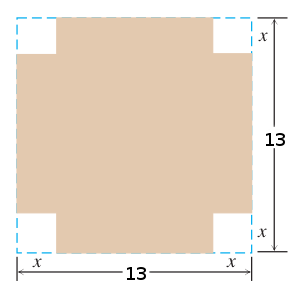
\includegraphics[scale=0.5]{./gc-termtestB-v1-01.png}
\end{figure}

\aufgabe{5} Evaluate the following limit.
\begin{equation}
\label{eq:voolohqu}
im_{x
ightarrowrac{pi}{2}}rac{2x-pi}{s{}x}\notag
\end{equation}

\end{document}
